\chapter{导数的概念}\label{ch:2.1}

各位同学大家好,本章我们进入可微性的分析当中,而其基础就是大家熟悉得不能再熟悉的导数。各位同学或许会觉得高中学过导数,也学过导函数,这一节就不学了,但是事实并非如此:
% enumerate空行比较大,考虑最终版更换环境
\begin{enumerate}
	\item 在填空题中,你会经常需要选择定义法或者导函数法;
	\item 一些导数的题目会披着\textbf{极限的外衣};
	\item 可导与否经常成为解题的前提与先决条件,探讨连续、可导、导函数的连续性也是常考题型;
	\item 导数几何意义中的求切线是常考题型;
	\item 对于一些特殊函数可导性的研究也经常出现选择题的中档题型。
\end{enumerate}

所以我希望同学们在本章打好基础,戒骄戒躁,继续保持刻苦学习的态度。

现对本节的排布进行说明:

\begin{enumerate}
	\item 学习(复习)导数的概念,一定要深刻理解,打好多变量函数导数的基础;
	\item 导数的几何意义一般以求切线的形式给出;
	\item 理解连续、可导、可微之间的关系,记忆一些可导而导函数不连续的状况;
	\item 进行模型、套路、题型的强化。
\end{enumerate}

\section{导数的定义}\label{sec:1.1}

\subsection{导数的引入}\label{sec:1.1.1}

大家高中时候都学过:对于位移函数,导数就是速度,因此某一位置的速度写为

\begin{equation*}
	v(t_o)=\underset{\Delta t\rightarrow 0}{\lim}\frac{s(t_0+\Delta t)-s(t_0)}{\Delta t}
\end{equation*}

某一不均匀质量的细棍的质量的导数,就是某一位置的线密度,因此某一位置的线密度写为

\begin{equation*}
	\rho(x_o)=\underset{\Delta x\rightarrow 0}{\lim}\frac{m(x_0+\Delta x)-s(x_0)}{\Delta x}
\end{equation*}

因此我们可以抽象出:对于某个函数在$x_0$处的导数\mn{在导数定义式中:
	\begin{enumerate}
		\item 微小变量需要可正可负;
		\item 分子分母的微小变量的表达式未必相同,但是极限值需要是1。
\end{enumerate}},就是

\begin{equation*}
	\underset{\Delta x\rightarrow 0}{\lim}\frac{\Delta y}{\Delta x}=\underset{\Delta x\rightarrow 0}{\lim}\frac{f(x_0+\Delta x)-f(x_0)}{\Delta x}
\end{equation*}

\begin{remark}
	这里给出了导数定义的第一个注意点:$\frac{f\qty(x_0+\text{微小变量})-f(x_0)}{\text{微小变量}}$,这个微小变量可证可负,在各种习题中未必会以$\lim\limits\Delta x\rightarrow 0$的形式出现,还有比如$\underset{x\rightarrow \infty }{\lim }\frac{1}{x}$。
\end{remark}

\subsection{导数的定义}\label{sec:1.1.2}

\subsubsection{导数}\label{sec:1.1.2.1}

\begin{definition}
	设函数$f$定义在$x_0$的某一\textbf{邻域}$U(x_0)$内,在此邻域内,当自变量$x_0$有改变量在$x_0$处该变量$\Delta x$时,相应地有函数$\Delta  y=f(x_0+\Delta x)-f(x_0)$.若当$\Delta x\rightarrow 0$时这两个改变量之比的极限
	\begin{equation}
		\underset{\Delta x\rightarrow 0}{\lim}\frac{\Delta y}{\Delta x}=\underset{\Delta x\rightarrow 0}{\lim}\frac{f(x_0+\Delta x)-f(x_0)}{\Delta x}\label{eq:1.1}
	\end{equation}
	存在,则称函数$f$在$x_0$可导,称\textbf{此比值的极限为$f$在$x_0$处的导数}。
\end{definition}

\begin{remark}
	这里给出了导数定义的第二个注意点:导数是比值的极限!既然导数是极限,极限就可以不存在,也可以无穷大——当极限不存在,称不可导;当极限为无穷大时,\textbf{虽然称极限不存在},但是不说导数不存在,就事论事,说导数为无穷大。
\end{remark}

\subsubsection{单侧导数}\label{sec:1.1.2.2}

上面提到:\textbf{微小变量$\Delta x$可正可负},那么如果为正,我们称为右导数;如果为负,称之为左导数。左右之分来自几何意义的:加上正变化,右面减左面;减去正变化,左面减右面,即

\begin{align*}
	&\text{右导数:}\underset{\Delta x\rightarrow 0^+}{\lim}\frac{f(x_0+\Delta x)-f(x_0)}{\Delta x}\\
	&\text{左导数:}\underset{\Delta x\rightarrow 0^-}{\lim}\frac{f(x_0+\Delta x)-f(x_0)}{\Delta x}
\end{align*}

\subsubsection{函数可导}

\begin{theorem}
	当函数$f(x)$的左右导数存在且相等时,称$f(x)$可导。
\end{theorem}

进一步,若$f(x)$在$x_0$处可导,则有$f(x)$在$x_0$处可微、$f(x)$在$x_0$连续。下作详细说明:

左导数存在说明左连续,右导数存在说明右连续,左右导数均存在说明函数连续,左右导数存在且相等说明函数可导。

\textbf{可导不可推出的结论}有:

\begin{enumerate}
	\item $f(x)$在$x_0$的某邻域内连续;
	\item $f'(x)$在$x_0$连续;
	\item $\underset{\Delta x\rightarrow x_0}{\lim}f'(x)$极限存在。
\end{enumerate}

取函数
$$ f(x)=\left\{
\begin{aligned}
	&0,&\text{$x$为有理数}\\
	&x^2,&\text{$x$为无理数}
\end{aligned}
\right.
$$

可以说明“不可推出结论”中的1。

取函数
$$ f(x)=\left\{
\begin{aligned}
	&x^2 \sin\frac{1}{x},&x\neq 0\\
	&0,&x=0
\end{aligned}
\right.
$$

可以说明“不可推出结论”中的2和3,此函数在0处可导但是导函数不连续,具体证明参考\textcolor{lbexacolor}{\nameref{sec:1.1.4.2}}\mn{点击红字即可跳转至相应位置}。

\subsection{导函数的定义}\label{sec:1.1.3}

请大家注意,直到这里,讲义的说法都是“此某一位置的速度、某一位置的线密度、某个函数于$x_0$处的导数”,而不是整个区间上的导数,因为导数的存在当然是有条件的,要从导数进入导函数,一定需要加入处处可导的条件,这是导函数存在\mn{因为某点的导数值就是导函数某点的值,所以导函数在题目中常常直接说成导数,不用太区分。}的\textbf{前决条件}。

\begin{definition}
	如果函数$f$在区间$I$上处处可导,对于每个$x$所生成的导数,我们称为$f'$,也就是导函数(非正式定义)。
\end{definition}

\subsection{导数的计算与求解}\label{sec:1.1.4}

\subsubsection{常见导数的计算}\label{sec:1.1.4.1}

高中阶段学过一些导数公式,为了帮助各位同学熟悉方法,我试着做以下计算\mn{熟悉极限运算的同学应该可以从一下证明中看到一些常见套路。}:

\begin{enumerate}
	\item 对于$\sin(x)$,熟知$\sin(x)-\sin(y)=2\cos(\frac{x+y}{2})\sin(\frac{x-y}{2})$. 
	
	故
	\begin{align*}
		\sin'(x)&=\underset{\Delta x\rightarrow 0}{\lim}\frac{\sin(x+\Delta x)-\sin(x)}{\Delta x}=\underset{\Delta x\rightarrow 0}{\lim}\frac{2\cos(\dfrac{x+\Delta x-x}{2})\sin(\dfrac{x-\Delta x-x}{2})}{\Delta x}\\
		&=\underset{\Delta x\rightarrow 0}{\lim}\frac{2\sin(\dfrac{\Delta x}{2})}{\Delta x}\cos(\frac{2x+\Delta x}{2})=\underset{\Delta x\rightarrow 0}{\lim}\cos(x+\frac{\Delta x}{2})=\cos(x)
	\end{align*}
    \item 对于$\cos(x)$,容易知道有$\cos(x)=\sin(x+\frac{\pi}{2})$,则自证不难。
    \item 对于$a^x=\underset{\Delta x\rightarrow 0}{\lim}\frac{a^{x+\Delta x}-a^x}{\Delta x}=\underset{\Delta x\rightarrow 0}{\lim}a^x\cdot\frac{a^{\Delta x}-1}{\Delta x}$,再令$a^{\Delta x}-1=t$,则$\Delta x=\log_a(1+t)=\frac{\ln(1+t)}{\ln a}$,替换,得原式$\underset{\Delta x\rightarrow 0}{\lim}a^x\cdot\frac{t\cdot \ln a}{\ln(1+t)}=a^x\ln a$。
    \item 对于$x^{\mu}$,有$x^{'\mu}=\underset{\Delta x\rightarrow 0}{\lim}\frac{(x+\Delta x)^{\mu}-x^{\mu}}{\Delta x}=\underset{\Delta x\rightarrow 0}{\lim}x^{\mu}\cdot \frac{(1+\dfrac{\Delta x}{x})^{\mu}-1}{\Delta x}=\underset{\Delta x\rightarrow 0}{\lim}x^{\mu}\cdot\mu\frac{\Delta x}{x}=\underset{\Delta x\rightarrow 0}{\lim}\mu x^{\mu-1}$
\end{enumerate}

\subsubsection{典型习题:探讨导数的存在性+导数的性质}\label{sec:1.1.4.2}

\begin{example}
	考察此函数的可导性。 
	$$ f(x)=\left\{
	\begin{aligned}
		&x \sin\frac{1}{x},&x\neq 0\\
		&0,&x=0
	\end{aligned}
	\right.
	$$
	\begin{enumerate}[label=(\arabic*)]
		\item 连续性讨论:$-|x|\le\underset{\Delta x\rightarrow 0}{\lim}f(x)\ge|x|\mbox{故}\underset{\Delta x\rightarrow 0}{\lim}=f(0)$,连续性成立。
		\item $\underset{\Delta x\rightarrow 0}{\lim}\frac{f(0+\Delta x)-f(0)}{\Delta x}=\underset{\Delta x\rightarrow 0}{\lim}\frac{\Delta x\sin\frac{1}{x}}{\Delta x}=\sin\frac{1}{\Delta x}$,\textbf{极限不存在},故不可导。
	\end{enumerate}
\end{example}\label{exa:}

\begin{example}
	讨论此函数在0处的连续、可导、导函数的连续性。
	$$ f(x)=\left\{
	\begin{aligned}
		&x^2 \sin\frac{1}{x},&x\neq 0\\
		&0,&x=0
	\end{aligned}
	\right.
	$$
	\begin{enumerate}[label=(\arabic*)]
		\item 参考\textcolor{lbexacolor}{\sffamily{例 1.1}} (1);
		\item $\underset{\Delta x\rightarrow 0}{\lim}\frac{f(0+\Delta x)-f(0)}{\Delta x}=\underset{\Delta x\rightarrow 0}{\lim}\frac{\Delta x^2\sin\dfrac{1}{x}}{\Delta x}=x\cdot\sin\frac{1}{\Delta x}=0$,\textbf{极限存在},故可导。
		\item $f'(x)=\sin\frac{1}{x}+x\cdot\frac{-1}{x^2}\cos(\frac{1}{x})$,显然$\underset{\Delta x\rightarrow 0}{\lim}f'(x)\neq f'(0)$,所以导函数存在但不连续。
	\end{enumerate}
\end{example}

\begin{marginfigure}[7em]
	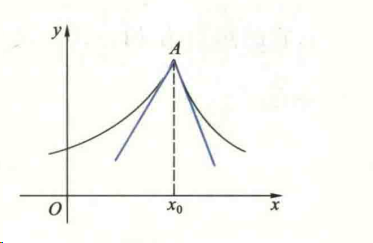
\includegraphics[width=\marginparwidth]{figures/screenshot001.png}
	\caption{$A$点两侧的切线}
	\label{fig:1.1}
\end{marginfigure}

\section{导数的几何意义}\label{sec:1.2}
因为高中接触切线比较多,此处不再多讲。

\subsection{几个切线的例子}\label{sec:1.2.1}

\subsubsection{左右导数存在却不相等}\label{sec:1.2.1.1}

\begin{marginfigure}[7em]
	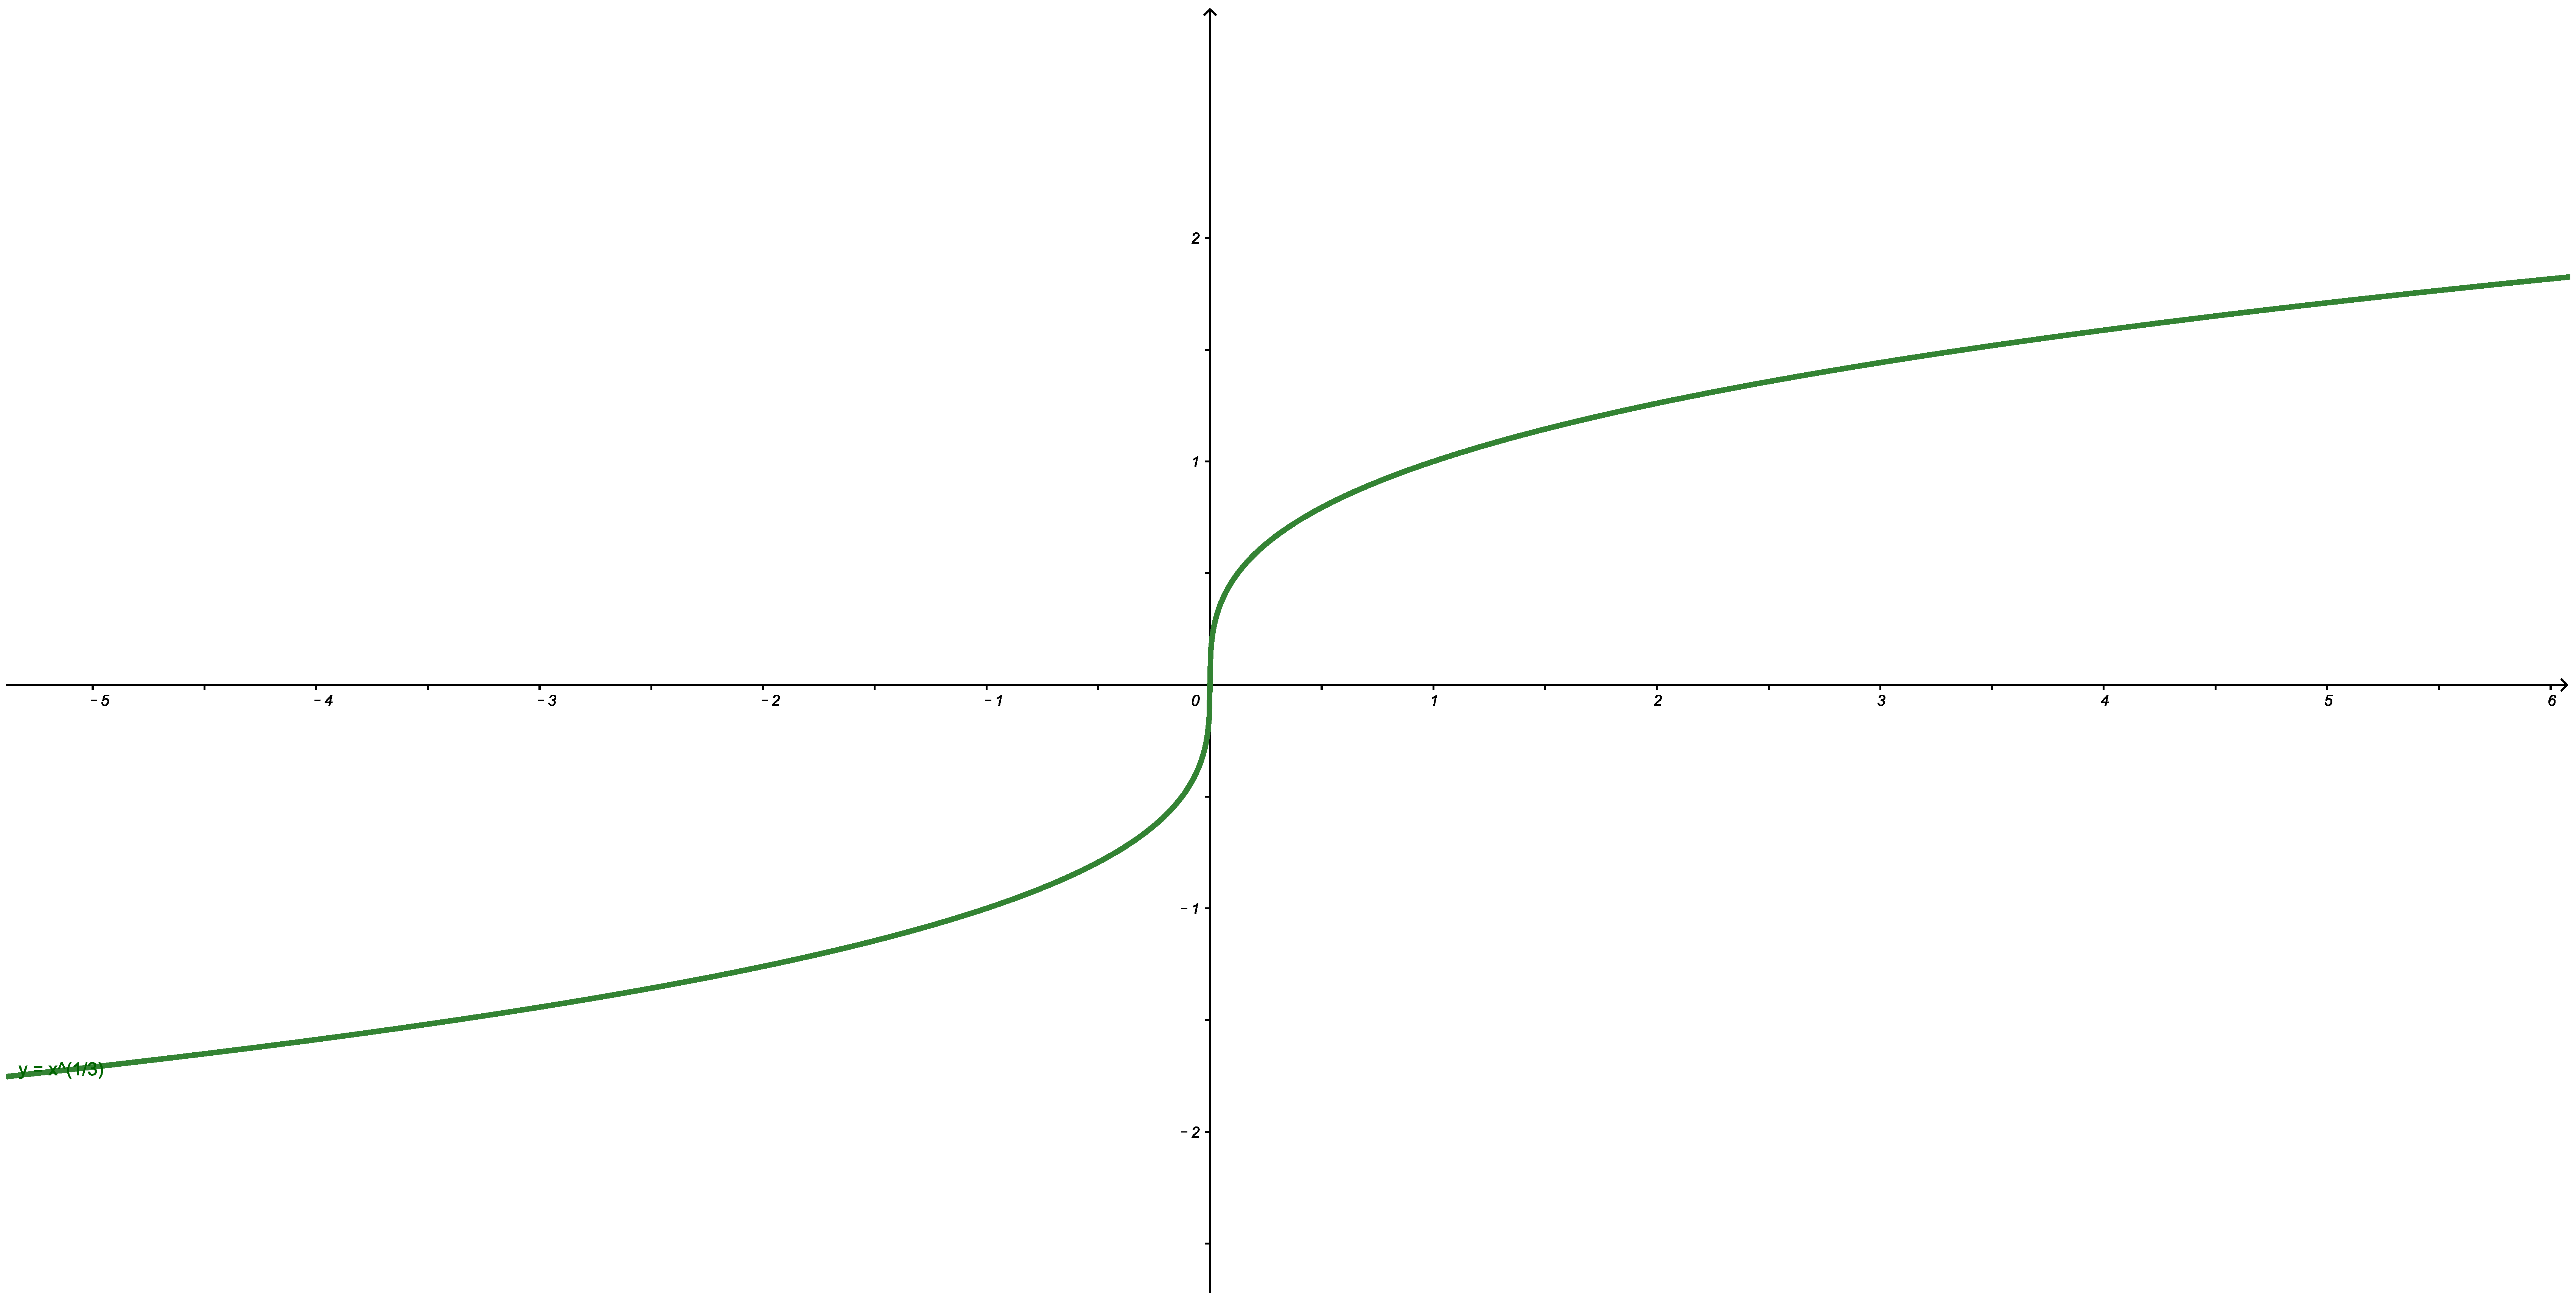
\includegraphics[width=\marginparwidth]{figures/2.eps}
	\caption{$O$点处的导数为正无穷}
	\label{fig:1.2}
\end{marginfigure}

高中学过,对于\textbf{可导函数},函数的导数在几何上表示曲线$y=f'(x)$在某点处的切线斜率。

对于\textbf{单侧导数存在的不可导函数},就把上面的表述更改为:\textbf{某侧导数表示某侧切线的斜率}。

图\ref{fig:1.1}所示的函数曲线,正好代表了某点在不同侧的切线,两条切线的斜率代表左右侧的导数值。如果左右导数存在且相等,那么两条切线二合一。

\subsubsection{导数的大小为正无穷}\label{sec:1.2.1.2}

如图\ref{fig:1.2}中$O$点处所示。

\subsubsection{不可导且曲线震荡}\label{sec:1.2.1.3}

如图\ref{fig:1.3}所示。

\begin{marginfigure}[7em]
	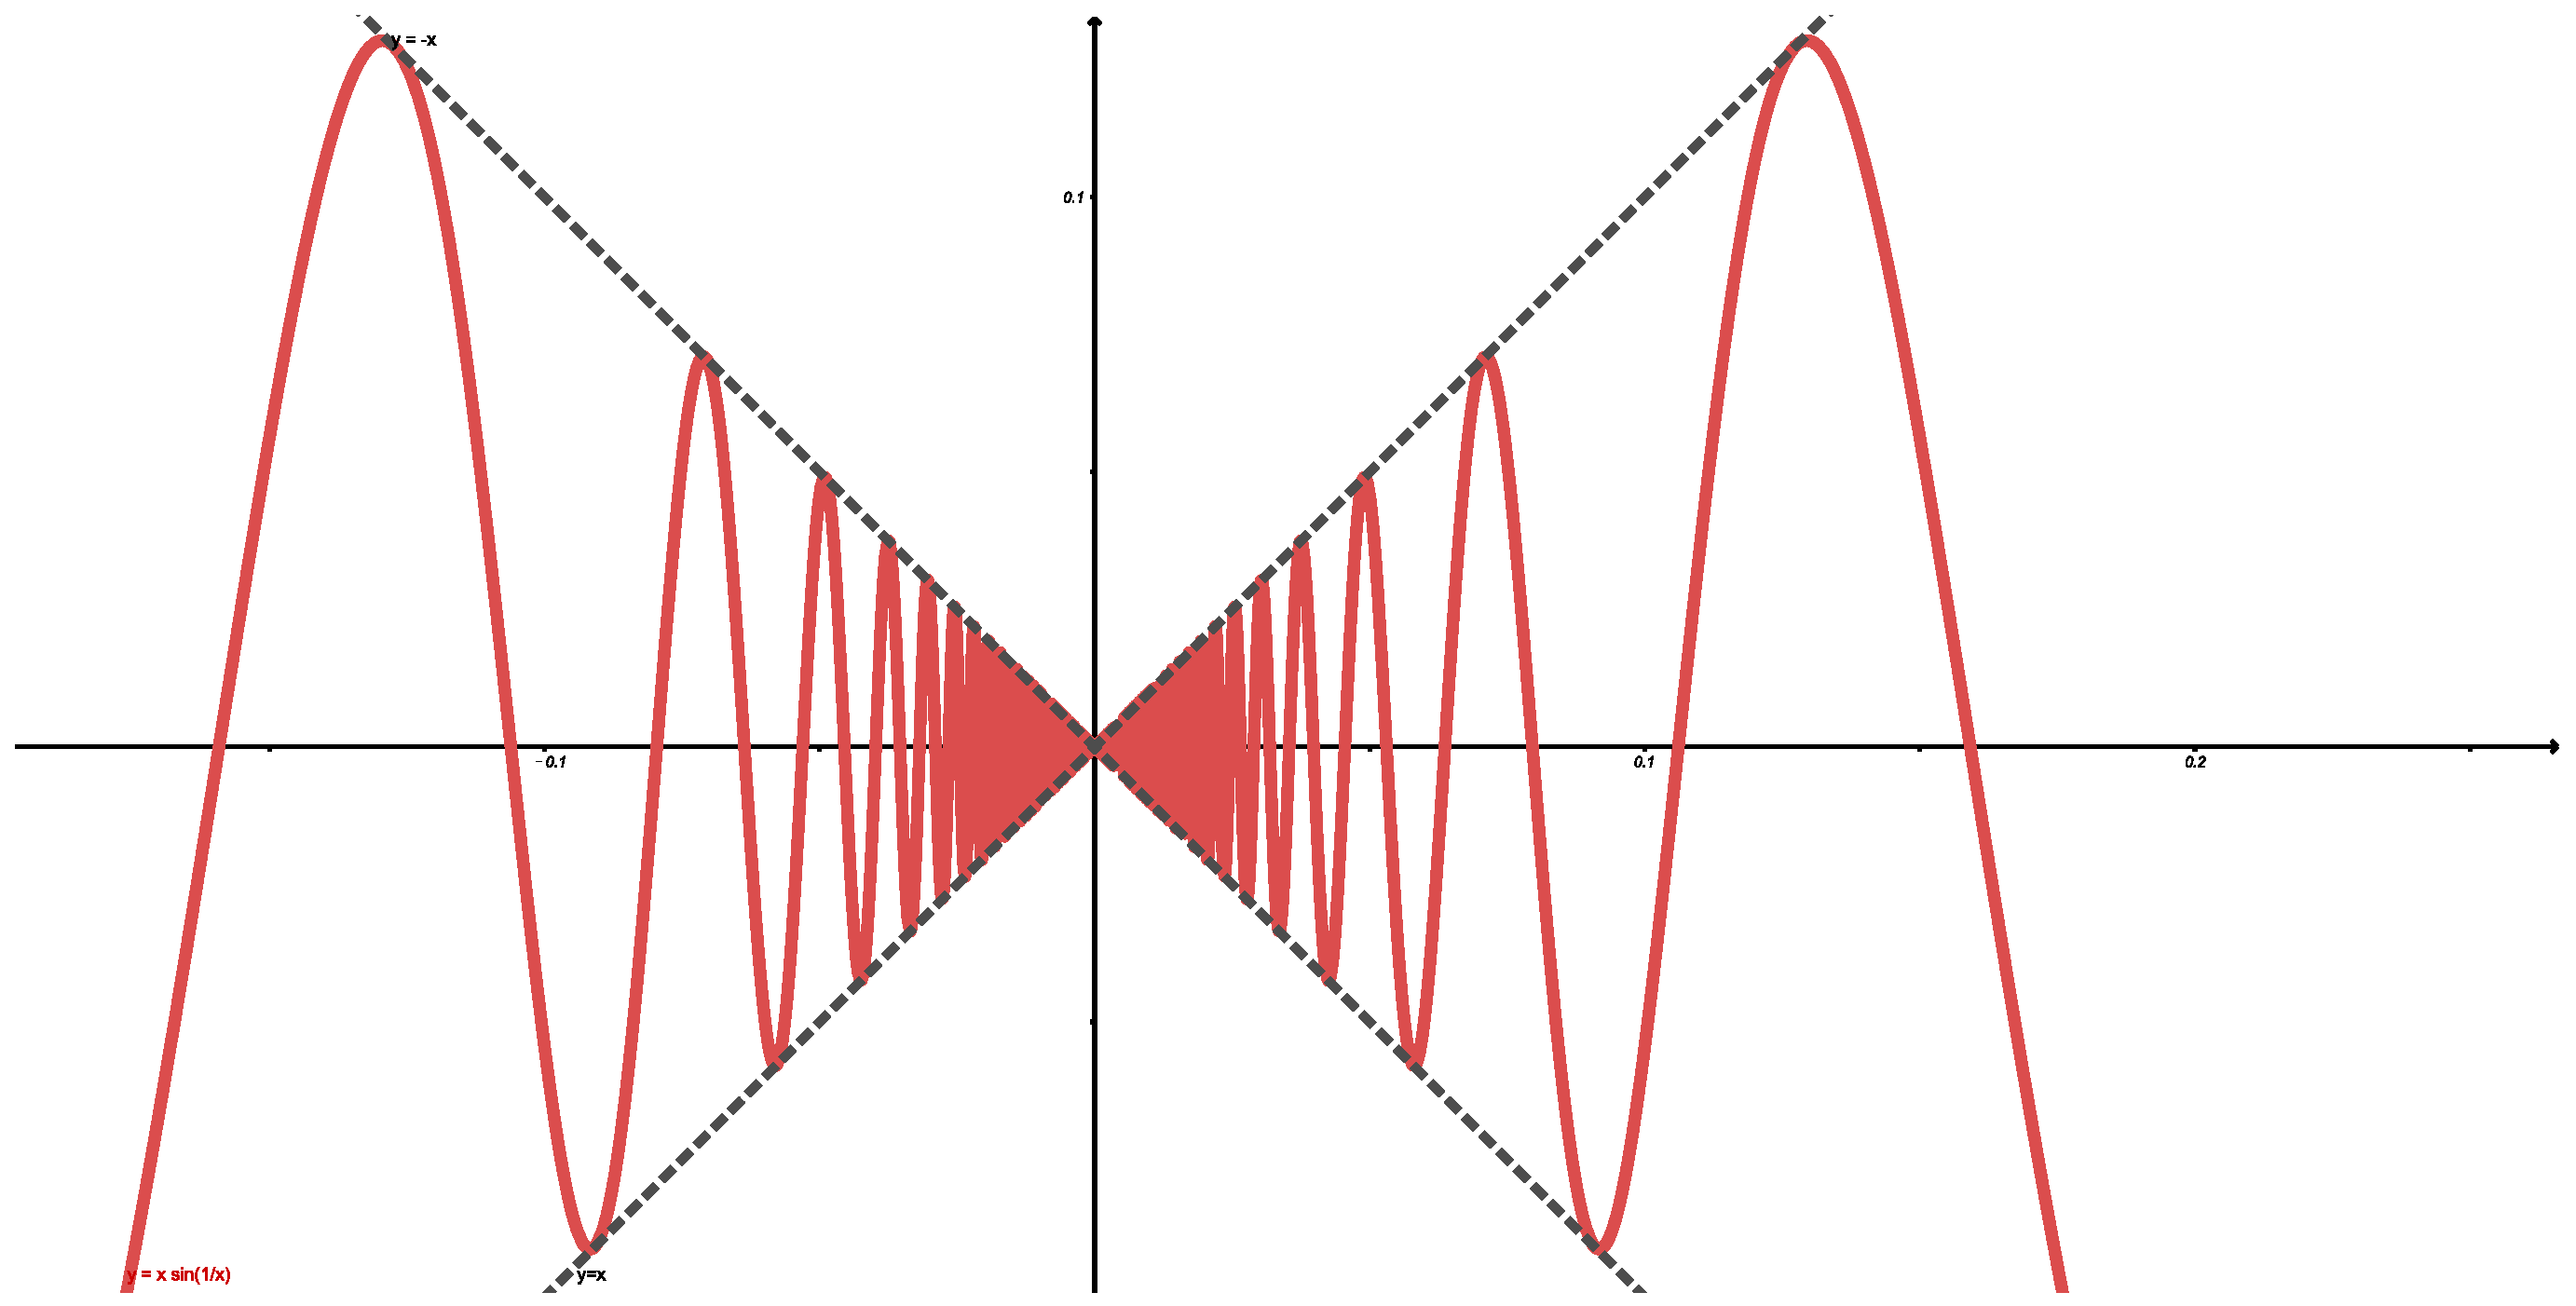
\includegraphics[width=\marginparwidth]{figures/3.eps}
	\caption{不可导且曲线震荡}
	\label{fig:1.3}
\end{marginfigure}

\section{模型、套路、题型}\label{sec:1.3}
\subsection{导数的存在}\label{sec:1.3.1}

\begin{problem}
	设$f(x)$在$x=0$处连续且$f(0)=0$,那么$f(x)$在$x=0$处可导的充分条件是\xparen
	\begin{xchoices}[showanswer = true]
		\item $\underset{\Delta x\rightarrow 0}{\lim}\frac{f(x)-f(-x)}{2x}$存在
		\item $\underset{\Delta x\rightarrow 0}{\lim}\frac{f\qty[\ln(1+x^2)]}{x^2}$存在
		\item $\underset{\Delta x\rightarrow 0}{\lim}\frac{f(x)}{\sqrt[3]{x}}$存在
		\item* $\underset{\Delta x\rightarrow 0}{\lim}xf\qty(\frac{1}{x})$
	\end{xchoices}
\vspace{0.5em}
\begin{solution}
	把握原则:“可导”$\Leftrightarrow$“左导数=右导数”。
	\begin{enumerate}[label=\Alph*.]
		\item 由$\underset{\Delta x\rightarrow 0}{\lim}\frac{f(x)}{x}$与$\underset{\Delta x\rightarrow 0}{\lim}\frac{f(-x)}{-x}$存在且相等$\Rightarrow\underset{\Delta x\rightarrow 0}{\lim}\frac{f(x)-f(-x)}{2x}$成立,但反之未必,此选项颠倒充分必要性。
		\item $\underset{\Delta x\rightarrow 0}{\lim} f(\ln(1+x^2))=\underset{\Delta x\rightarrow 0}{\lim}x^2\ge 0$因此不满足左右导数,只满足右导数。
		\item 显然不同阶。
		\item 如知识点叙述所说:$\underset{\Delta x\rightarrow \infty}{\lim}\frac{f(1/x)}{1/x}$存在,因此成立\mn{\textbf{总结反思:}在导数定义式中:
		\begin{enumerate}
			\item 微小变量需要可正可负;
			\item 分子分母的微小变量的表达式未必相同,但是极限值需要是1。
		\end{enumerate}}。
	\end{enumerate}
\end{solution}
\end{problem}
	
\subsection{导数与极限互化}\label{sec:1.3.2}

\begin{problem}
	设函数$y=f(x)$在点$x=0$处连续,且$\underset{\Delta x\rightarrow 0}{\lim}\frac{f(x)-2x}{1-\cos(x)}=1$,则在0处有\xparen
	
	\begin{xchoices}[showanswer = true]
		\item 不可导
		\item 可导且$f'(0)=0$
		\item 可导且$f'(0)=-2$
		\item* 可导且$\dd y\big|_{x=0} = 2\dd x$
	\end{xchoices}
	\vspace{0.5em}
	\begin{solution}
		\begin{enumerate}[label=(\Roman*)]
			\item 见到$1-\cos(x)$想到$\frac{1}{2}x^2$因此有$\underset{\Delta x\rightarrow 0}{\lim}\frac{2f(x)/x-4}{x}=1$,故有$\underset{\Delta x\rightarrow 0}{\lim}\frac{f(x)}{x}=2$,而显然$f(0)=0$,因此可导可微,且导数为2。
			\item $\underset{\Delta x\rightarrow 0}{\lim}f(x)=\frac{1}{2}x^2+2x$,故$\underset{\Delta x\rightarrow 0}{\lim}f'(x)=2+x$,所以可导,导数为2\mn{\textbf{总结反思:}由此题可以看出遇到这种形式的极限时,应该如何实现极限与导数的互化。解析中的思路(II)是编者自己第一次见到这个题目时候想到是不是能把表达式写出来,不一定对,如果不对请及时反映。}。
		\end{enumerate}
	\end{solution}
\end{problem}

\begin{problem}
	已知$f(x)$在$x=0$处连续,且$\underset{\Delta x\rightarrow 0}{\lim}[f(x)+e^x]^{\frac{1}{x}}=2$,则$f'(0)=$\xparen
	\begin{xchoices}[showanswer = true]
		\item 不存在
		\item $\ln(2)$
		\item $2$
		\item* $\ln(2)-1$
	\end{xchoices}
\vspace{0.9em}
    \begin{solution}
    	$\underset{\Delta x\rightarrow 0}{\lim}\frac{\ln[f(x)+e^x]}{x}=\ln2$\mn{取对数处理法是面对指数型极限的常用处理方式,由此题注意总结。},故$\underset{\Delta x\rightarrow 0}{\lim}\ln[f(x)+e^x]=0$,故$f(0)=0$,此时就形成了$\frac{f(x)}{x}$模型,而$\underset{\Delta x\rightarrow 0}{\lim}\frac{\ln[f(x)+e^x]}{x}=\underset{\Delta x\rightarrow 0}{\lim}\frac{f(x)+e^x-1}{x}=\ln2$,故得$f'(0)=-1+\ln(2)$。
    \end{solution}
\end{problem}

\begin{problem}
	对于$y=f(x)$,有$f(1)=0, f'(1)=1$,求$\underset{n\rightarrow \infty}{\lim}f\qty(\frac{n}{n+2})$的值。
	\begin{solution}
		显然属于极限导数互化,尝试构造$x=1$处的导数\mn{既然是已经给了某处的函数导数值,那就把它直接构造出来。}。
		$$
		\underset{n\rightarrow \infty}{\lim}n\cdot \frac{f\qty(1+\dfrac{-2}{n+2})-0}{\dfrac{-2}{n+2}\cdot\dfrac{n+2}{-2}}=\frac{-2n}{n+2}\cdot \underset{ n\rightarrow \infty}{\lim}f'(1)=-2
		$$
	\end{solution}
\end{problem}

\begin{problem}
	设$f(x)$在$x=a$处二阶可导,则极限$\underset{ x\rightarrow 0}{\lim}\frac{\dfrac{f(a+x)-f(a)}{x}-f'(a)}{x}=$\xparen
	\begin{xchoices}[showanswer = true]
		\item ${0}$
		\item ${f''(a)}$
		\item ${2f''(a)}$
		\item* ${\frac{f''(a)}{2}}$
	\end{xchoices}
\vspace{0.5em}
\begin{solution}
	第一眼看上去仿佛是:$\frac{f'(a)-f'(a)}{x}$,但是由于极限的:趋近而非完全相等的性质,需要进一步探究阶数与小量的关系。
	\begin{enumerate}[label=(\Roman*)]
		\item $\frac{f(a+x)-f(a)-xf'(a)}{x^2}$,进一步,由洛必达法则,有$\underset{ x\rightarrow 0}{\lim}\frac{f'(a+x)-f'(a)}{2x}=\frac{f''(a)}{2}$。
		\item $f(a+x)=f(a)+f'(a)x+\frac{f''(a)}{2!}x^2+o(x^2)$,则有$\underset{ x\rightarrow 0}{\lim}\frac{f(a+x)-f(a)-f'(a)x}{x^2}=\underset{ x\rightarrow 0}{\lim}\frac{\frac{f''(a)}{2}x^2+o(x^2)}{x^2}=\frac{f''(a)}{2}$\mn{认真体会思路(I)和(II)的区别与相通性:其实是洛必达与泰勒的相通性。}。
	\end{enumerate}
\end{solution}
\end{problem}

\subsection{可导性探源}\label{sec:1.3.3}

\begin{problem}
	已知函数$f(x) =\left|x-x^2\right|({\rm e}^x-1)+\sin|x-2|$的不可导点的个数为\xparen
	
	\begin{xchoices}[showanswer = true]
		\item 0
		\item 1
		\item* 2
		\item 3
	\end{xchoices}
	\vspace{0.5em}
	\begin{solution}
		不可导点一般模型有两种,此题为第一种,函数表达式明确。对于寻找不可导点,其实就是由外向内层层剥离函数。
		\begin{enumerate}[label=(\arabic*)]
			\item 简化函数表达式到最清晰的情况:$f(x)= |x||x-1|({\rm e}^x-1)+sin|x-2|$;
			\item 依次确定每个函数的特殊点\mn{对于绝对值形成的函数,可不可导的关键就是$\underset{\Delta x\rightarrow 0}{\lim}\frac{f(x+\Delta x)-f(x)}{\Delta x}$是否会因为绝对值的存在导致左右异号,此题中$|x|$函数因为有${\rm e}^x-1$的存在避免了这种情况。}:0、1、0、2;
			\item 对$x=0$,依据定义$\underset{ x\rightarrow 0}{\lim}\frac{f(x)-f(0)}{x}=\underset{\Delta x\rightarrow 0}{\lim}=\sin 2$,恒有左右导相等;
			\item 对$x=1$,依据定义$\underset{\Delta x\rightarrow 0}{\lim}\frac{f(1+\Delta x)-f(1)}{\Delta x}=\underset{\Delta x\rightarrow 0}{\lim}\pm|1+\Delta x|\qty({\rm e}^{|1+\Delta x|}-1)+\sin(-1+\Delta x)$,左右导不相等;
			\item 对$x=2$,同上,发现左右导数不相等。
		\end{enumerate}
	\end{solution}
\end{problem}

\begin{problem}
	$f(x)=\underset{ n\rightarrow \infty}{\lim}\sqrt[n]{1+|x|^n+{\rm e}^{nx}}$的不可导点个数为\xparen
	\begin{xchoices}[showanswer=true]
		\item 0
		\item 1
		\item* 2
		\item 3
	\end{xchoices}
\vspace{0.5em}
\begin{solution}
	此题的函数以极限形式出现,所以首先要给出不同区间上的函数表达式\mn{以极限形式出现的函数,要写出其具体形式,一般为分段函数。}。
	
	\begin{enumerate}[label=(\arabic*)]
		\item 对于$\underset{ n\rightarrow \infty}{\lim}{\rm e}^{nx}$,当$x\ge 0$时趋于正无穷,$x\le 0$时趋于0;
		\item 对于$\underset{ n\rightarrow \infty}{\lim}|x|^n$,当$x\in(-1,1)$时趋于0,反之趋于正无穷,但是是那种远小于${\rm e}^{nx}$的正无穷,证明即$\frac{|x|^n}{{\rm e}^{nx}}=\qty(\frac{x}{{\rm e}^x})^n=0$;
		\item 因此,由区间划分为
		$ f(x)=\left\{
		\begin{aligned}
			&-x,&x\le -1\\
			&1,&-1\leq x\geq 0\\
			&e^x,&x\ge 0
		\end{aligned}
		\right.
		$;
		\item 发现两个分界点:-1,0皆不可导。
	\end{enumerate}
\end{solution}
\end{problem}

\subsection{复杂求导方法与典型导数模型}\label{sec:1.3.4}

\begin{problem}
	已知$f(x)=\frac{(x-1)(x-2)...(x-n))}{(x+1)(x+2)...(x+n)}$,求$f'(1)$的值。
	\vspace{0.3em}
	\begin{solution}
		按部就班写出导数表达式,显然有$f(1)=0$,于是
		\begin{align*}
			f'(1)&=\underset{ x\rightarrow 1}{\lim}=\frac{\dfrac{(x-1)(x-2)...(x-n))}{(x+1)(x+2)...(x+n)}}{x-1}=\frac{(x-2)...(x-n))}{(x+1)(x+2)...(x+n)}\\
			&=\frac{(-1)^{n-1}(n-1)!}{(n+1)!}=\frac{(-1)^{n-1}}{n(n+1)}
		\end{align*}
	\end{solution}
\end{problem}

\begin{problem}
	已知$f(x)=\sqrt{\frac{(1+x)\sqrt{x}}{e^{x-1}}}$,求$f'(1)$的值。
	\begin{solution}
		显然采用对数求导法,按照如下格式。
		
		$\ln(g(x))=\frac{1}{2}[\ln(1+x)+\frac{1}{2}\ln(x)-(x-1)]$,$\frac{g'(x)}{g(x)}=\frac{1}{2}\qty(\frac{1}{x+1}+\frac{1}{2x}-1)$,$\frac{g'(1)}{g(1)}=0$,故$g'(1)=0$
	\end{solution}
\end{problem}